%------------------------------------------------------------
% DEFINITIONS AND HEADERS -- IGNORE THIS
%------------------------------------------------------------
\documentclass{article}
\usepackage[top=2.0cm, bottom=3cm, left=2.5cm, right=2.25cm]{geometry}
\usepackage[utf8]{inputenc}
\usepackage{algpseudocode}
% Get better typography
\usepackage[protrusion=true,expansion=true]{microtype}	
% For algorithms
\usepackage[boxruled,linesnumbered,vlined,inoutnumbered]{algorithm2e}
\SetKwInOut{Parameter}{Parameters}
% For basic math, align, fonts, etc.
\usepackage{amsmath}
\usepackage{amsthm}
\usepackage{amssymb}
\usepackage{mathtools}
\usepackage{mathrsfs}
\usepackage{rotating}
\usepackage{tabularx}
\usepackage{booktabs}
\usepackage{soul}
\usepackage{changepage}
\usepackage{gensymb} % For \degree
\usepackage{lscape}
% For \thead to make line breaks in tables
\usepackage{array}
\usepackage{makecell}
\renewcommand\theadalign{bc}
\renewcommand\theadfont{\bfseries}
\renewcommand\theadgape{\Gape[4pt]}
\renewcommand\cellgape{\Gape[4pt]}
\usepackage{courier} % For \texttt{foo} to put foo in Courier (for code / variables)
\usepackage{lipsum} % For dummy text
\usepackage{listings}
\lstset{
    basicstyle=\ttfamily\small,
    keywordstyle=\color{darkblue}\bfseries,
    commentstyle=\color{darkgreen},
    stringstyle=\color{darkred},
    frame=single,
    breaklines=true,
    columns=fullflexible,
    showstringspaces=false
}
% For images
\usepackage{graphicx}
\usepackage{subcaption}
\usepackage[space]{grffile} % For spaces in image names
% For bibliography
\usepackage[round]{natbib}
% For color
\usepackage{xcolor}
\definecolor{light-grey}{rgb}{0.9,0.9,0.9}
\definecolor{dark-red}{rgb}{0.4,0.15,0.15}
\definecolor{dark-blue}{rgb}{0,0,0.7}
\definecolor{darkblue}{rgb}{0,0,.6}
\definecolor{darkred}{rgb}{.58,0,0}
\definecolor{brighterred}{rgb}{.745,0,0}
\definecolor{darkgreen}{rgb}{0,.6,0}
\definecolor{red}{rgb}{.98,0,0}
\usepackage{environ}
% Only show sections in table of contents and rename
\setcounter{tocdepth}{2}
\renewcommand{\contentsname}{Table of Contents}
% For links (e.g., clicking a reference takes you to the phy)
\usepackage{hyperref}
\hypersetup{
    colorlinks, linkcolor={dark-blue},
    citecolor={dark-blue}, urlcolor={dark-blue}
}
\newcommand{\TODO}[1]{\textcolor{blue}{\textbf{{#1}}}}
\newcommand{\POINTS}[1]{\textcolor{purple}{\textbf{{#1}}}}
\providecommand{\mathcolor}[2]{\textcolor{#1}{#2}}
% My definition of "summary boxes" (see below)
\usepackage[most]{tcolorbox}
\definecolor{boxgray}{rgb}{0.95, 0.95, 0.95}
\definecolor{boxblue}{rgb}{0.941, 0.941, 0.98}
\definecolor{boxpink}{rgb}{1.0, 0.93, 0.93}
\definecolor{boxwhite}{rgb}{1.0, 1.0, 1.0}
%\definecolor{boxgreen}{rgb}{0.91, 0.96, 0.9}
\definecolor{boxgreen}{rgb}{0.92, 0.96, 0.92}
\newtcolorbox{mybox}[1][boxwhite]{%
  enhanced,
  boxrule=0.5pt,
  colframe=black,
  colback=#1,
  sharp corners,
  width=\linewidth,
  left=1em,
  right=1em,
  top=0.5em,
  bottom=0.5em,
  boxsep=0pt,
  before skip=1em,
  after skip=0.85em,
}
%------------------------------------------------------------








\begin{document}
%-----------------
%	Homework 5
%-----------------
\newpage
\vspace*{1cm}
\begin{center}
    \begin{Large}
    COMPSCI 687 Homework 5 - Fall 2025
    \end{Large}
    \\
    \vspace{0.15cm}
    Due \textcolor{darkred}{\textbf{December 1}}, 11:55pm Eastern Time
\end{center}
\addcontentsline{toc}{subsection}{\textbf{Homework 5}}



\vspace{1.0cm}
\section{Instructions}

\begin{itemize}
    \item This homework consists only of a programming part.
    \item While you may discuss problems with your peers (e.g., to discuss high-level approaches), you must answer the questions on your own. In your submission, do explicitly list all students with whom you discussed this assignment. 
    \item Submissions must be typed. You must use \LaTeX. Handwritten and scanned submissions will not be accepted. 
    \item The assignment should be submitted on Gradescope as a PDF with marked answers via the Gradescope interface. The source code should be submitted via the Gradescope programming assignment as a .zip file. Include with your source code instructions for how to run your code. You \textbf{must} use Python 3 for your homework code. 
    \item You may \underline{not} use any reinforcement learning or machine learning specific libraries in your code, e.g., TensorFlow, PyTorch, or scikit-learn. You \textit{may} use libraries like numpy and matplotlib, though.
    \begin{itemize}
    \item You must write your own code from scratch. 
    \item \textbf{The only exception is that you may re-use code you wrote for previous homework assignments. }
    \item \textcolor{darkred}{We will use an automated system to detect plagiarism.} Your code will be compared against submissions from your classmates as well as publicly available implementations online.
    \end{itemize}
    \item The automated system will not accept assignments after 11:55pm on December 1. 
    \item The .tex file for this homework can be found on Canvas under ``\textit{Homework \#5 - Supporting Files}''. 
\end{itemize}





%------------------------------------------------------------------------
%  PROGRAMMING / CODING SECTION
%------------------------------------------------------------------------
\newpage



%---- Intro and Problem Specification ----------------------    
\vspace*{-0.75cm}
\section*{Programming Assignment \POINTS{[100 Points, total]}}
\vspace{0.25cm}

\looseness-1
In this assignment, you will implement three algorithms based on Temporal Difference (TD): TD-Learning for policy evaluation, and SARSA and Q-Learning for policy optimization. You will deploy all three algorithms on the Cat-vs-Monsters domain. A complete definition of the Cat-vs-Monsters domain can be found in Homework 3.

\begin{mybox}[boxpink] 
\textbf{Notice that you may \underline{not} use existing RL code for this problem. You must implement the agent and environment entirely on your own and from scratch.} 
\end{mybox}


\vspace{0.15in}
\begin{mybox}[boxblue] 
\textbf{General instructions:}
\begin{itemize}
    \item You are free to initialize the $q$-function in any way that you want. More details about this later. 
    \item Whenever displaying values (e.g., the value of a state), use 4 decimal places; e.g, $v(s)=9.4312$.
    \item Whenever showing the value function and policy learned by your algorithm, present them in a format resembling that depicted in Figure \ref{fig:v_pi_star_cat_monsters}.
\end{itemize}
\end{mybox}

\begin{figure}[!!hb]
    \centering
    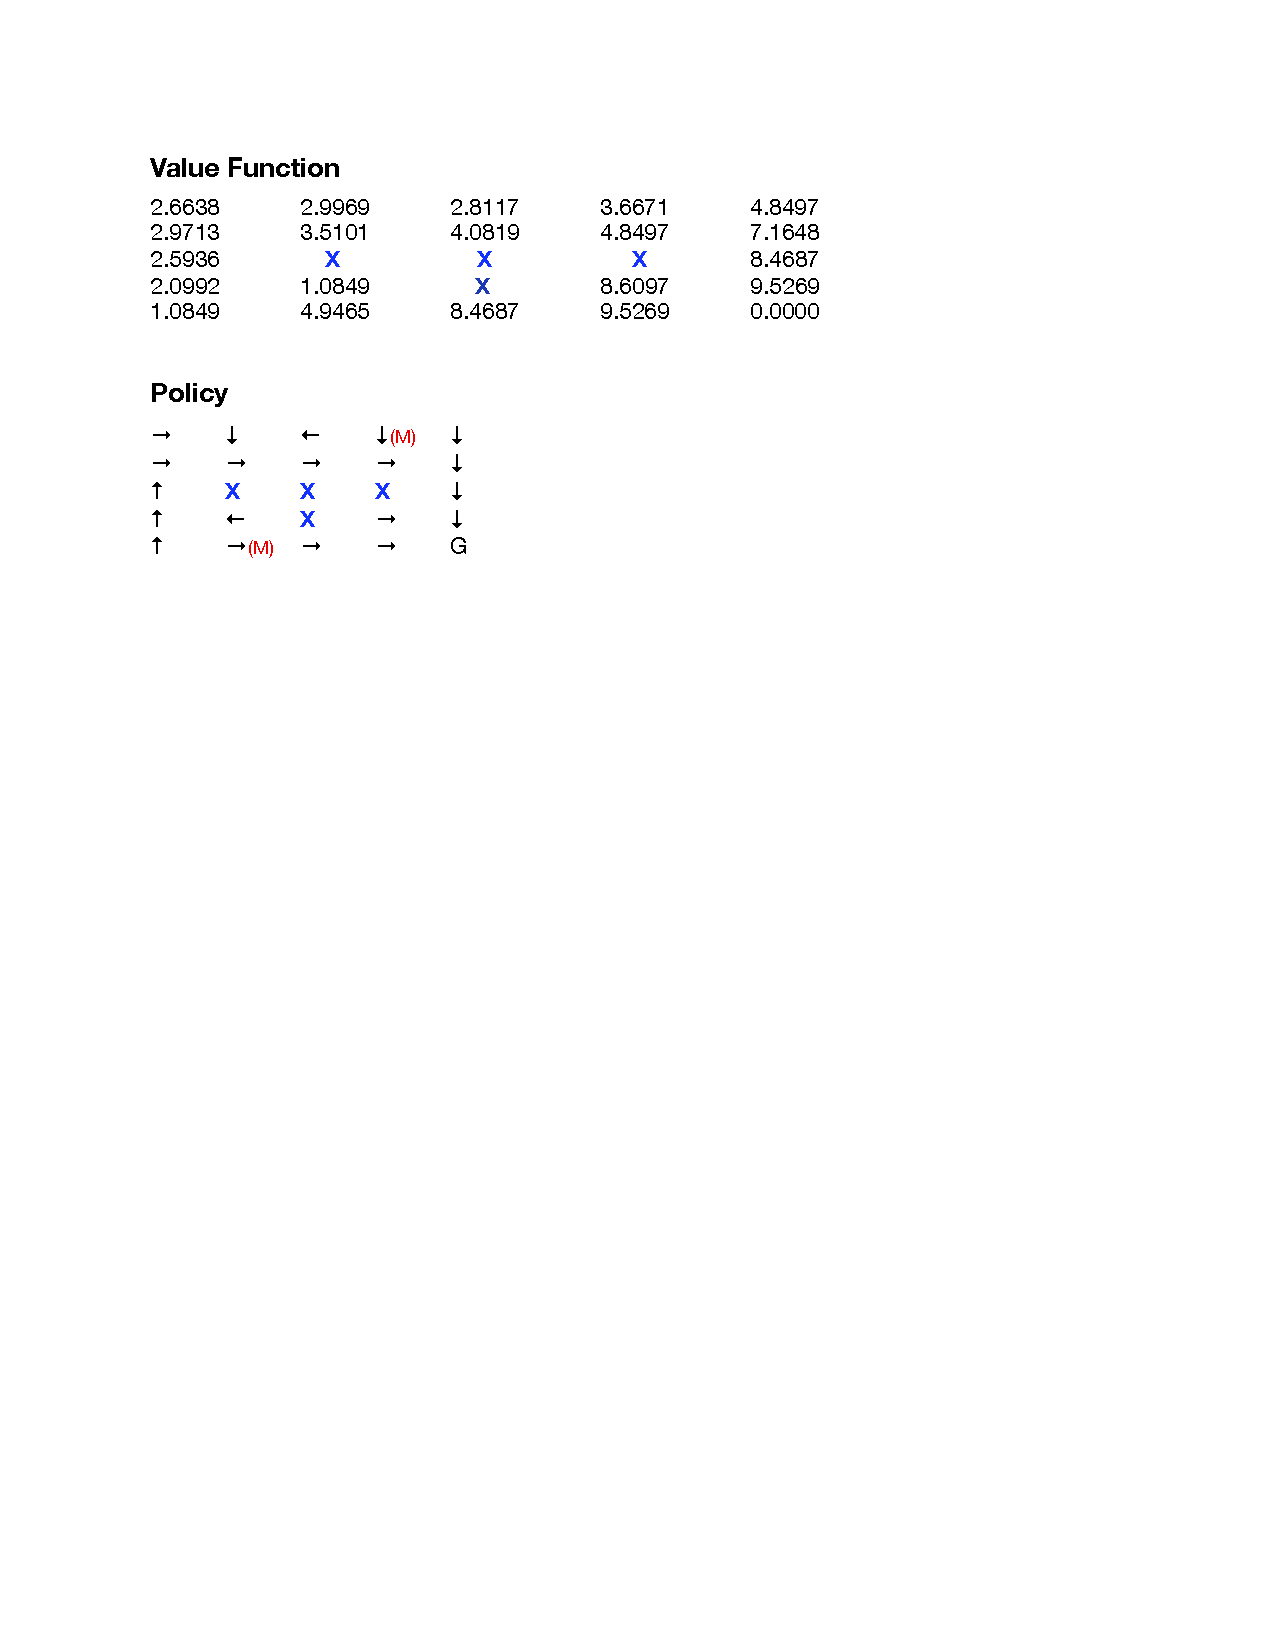
\includegraphics[width=0.5\textwidth]{HW_figs/v_pi_star_cat_monsters.pdf}
    \caption{Optimal value function and optimal policy for the Cat-vs-Monsters domain.}
    \label{fig:v_pi_star_cat_monsters}
\end{figure}

\vspace{0.7cm}






%---- Question 1 ----------------------

\noindent {\Large{\textbf{1.} \textbf{TD-Learning in the Cat-vs-Monsters domain} \POINTS{[20 Points, total]}}}
\vspace{0.4cm}
    
\noindent First, implement the TD-Learning algorithm for policy evaluation and use it to learn an estimate, $\hat{v}$, of the value function of the optimal policy, $\pi^*$, for the Cat-vs-Monsters domain. \textbf{Remember that both the optimal value function and the optimal policy for the Cat-vs-Monsters domain were identified in a previous homework using the Value Iteration algorithm. For reference, both are shown in Figure \ref{fig:v_pi_star_cat_monsters}.} When sampling trajectories, set $d_0$ to be a uniform distribution over $\mathcal{S}$ to ensure that you are collecting returns from all states. Do not allow the agent to be initialized in a Forbidden Furniture location. Note that using this alternative definition of $d_0$ (instead of the original one) is important because we want to generate trajectories from all states in the MDP, not just those visited under the optimal deterministic policy shown in Figure \ref{fig:v_pi_star_cat_monsters}.
\vspace{0.2cm}
    
\noindent You should run your algorithm until the value function estimate does not change significantly between successive iterations; i.e., whenever the Max-Norm between $\hat{v}_{t-1}$ and $\hat{v}_t$ is at most $\delta$, for some value of $\delta$ that you should set empirically. For each run of your algorithm, count how many episodes were necessary for it to converge to an estimate of $v^{*}$. Run your algorithm, as described above, 50 times, and then:

\newpage
\begin{itemize}


        %---- Question 1a ----------------------
        \item \textbf{(Question 1a.~\POINTS{3 Points})} Report the value of $\alpha$ that you used. You should choose a value of $\alpha$ that allows the algorithm to converge to a solution close to $v^{*}$, without requiring an excessively large number of episodes.
        \vspace{0.2cm}
        \textbf{Answer.} I selected $\alpha = 0.18$ after running TD(0) with $\alpha \in \{0.10, 0.14, 0.18, 0.22\}$, fixing $\delta = 10^{-4}$, a minimum of 500 episodes, and a maximum of 6{,}000 episodes per run. $\alpha = 0.18$ was the first value that consistently converged to within the target max-norm tolerance without pushing the variance of the episode counts too high. Smaller stepsizes converged cleanly but required noticeably more rollouts, while $\alpha \geq 0.22$ introduced mild oscillations around the monster-adjacent cells.



        %---- Question 1b ----------------------
        \item \textbf{(Question 1b.~\POINTS{10 Points})} Report the average value function estimated by the algorithm, that is, the average of all 50 value functions learned by the algorithm at the end of its execution. Also report the Max-Norm between this average value function and the optimal value function for the Cat-vs-Monsters domain.
        \vspace{0.2cm}
        \textbf{Answer.} Table~\ref{tab:td_value} lists the element-wise average of the 50 post-convergence value functions, rounded to four decimals. The grid is reported in the same north-to-south orientation used in Homework~3 (row~5 is the top corridor, row~1 contains the goal). Forbidden furniture squares are marked with ``X''. The averaged estimate stays within $0.6774$ max-norm distance of the optimal value table computed via Value Iteration.

        \begin{table}[h]
            \centering
            \caption{Average value function $\bar v$ learned by TD(0) after 50 runs.}
            \label{tab:td_value}
            \begin{tabular}{c|ccccc}
                & $c=1$ & $c=2$ & $c=3$ & $c=4$ & $c=5$\\
                \hline
                $r=5$ & 2.8218 & 3.1523 & 2.9763 & 2.9897 & 4.9969\\
                $r=4$ & 3.1367 & 3.7283 & 4.2959 & 5.1924 & 7.3295\\
                $r=3$ & 2.7775 & X & X & X & 8.4791\\
                $r=2$ & 2.2771 & 1.0131 & X & 8.5868 & 9.5298\\
                $r=1$ & 1.0681 & 5.2774 & 8.5755 & 9.6237 & 0.0000\\
            \end{tabular}
        \end{table}



        %---- Question 1c ----------------------
        \item \textbf{(Question 1c.~\POINTS{7 Points})} Report the mean and standard deviation of the number of episodes required for the algorithm to converge.
        \vspace{0.2cm}
        \textbf{Answer.} Across the 50 independent runs, TD(0) needed on average $516.7$ episodes to satisfy the convergence test, with a standard deviation of $14.5$. The narrow spread reflects both the fixed exploration distribution (uniform over non-forbidden cells) and the relatively conservative $\alpha = 0.18$.


        
\end{itemize}
    





%---- Question 2 ----------------------    

\vspace{0.75cm}
\noindent {\Large{\textbf{2.} \textbf{SARSA in the Cat-vs-Monsters domain} \POINTS{[40 Points, total]}}}
\vspace{0.4cm}

\noindent Implement the SARSA algorithm and use it to learn $\hat{q}$, an estimate of the optimal action-value function, $q^{*}$, for the Cat-vs-Monsters domain; and to learn an estimate, $\hat{\pi}$, of its optimal policy, $\pi^*$. You will need to make four main design decisions: \textit{(i)} which value of $\alpha$ to use; \textit{(ii)} how to initialize the $q$-function; you may, for example, initialize it with zeros, with random values, or optimistically. Recall that $q(s_\infty, \cdot) = 0$ by definition; \textit{(iii)} how to explore; you may use different exploration strategies, such as $\epsilon$-greedy or softmax action selection; and \textit{(iv)} how to control the exploration rate over time; you may choose to keep the exploration parameter (e.g., $\epsilon$) fixed or have it decay as a function of the number of episodes. 
\vspace{0.3cm}

\begin{itemize}


    %---- Question 2a ----------------------
    \item \textbf{(Question 2a.~\POINTS{4 Points})} Report the design decisions \textit{(i--iv)} that you made, and discuss the reasoning behind each of your choices.
    \vspace{0.2cm}
    \textbf{Answer.} My final configuration balanced stability and exploration as follows:
    \begin{itemize}
        \item \textbf{Step-size ($\alpha$).} Set to $0.25$. This was the largest value that kept the tabular updates stable even when an episode spent many steps dodging monsters. Smaller values converged, but the learning curves flattened later.
        \item \textbf{Initialization.} All $q$-values started at $+1.0$ (the absorbing goal remained at $0$). This mild optimistic initialization nudged the agent to leave the safe western corridor during the first 50--75 episodes.
        \item \textbf{Exploration.} Plain $\epsilon$-greedy was sufficient. The stochasticity of the domain plus optimistic $q$-values already injects variety; more complex schemes (softmax with temperature schedules) did not improve convergence.
        \item \textbf{Exploration schedule.} $\epsilon$ began at $0.30$ and decayed multiplicatively by $0.995$ per episode down to $0.02$. This lets the policy explore broadly for roughly 150 episodes, then exploit once the value estimates stabilize.
    \end{itemize}



    %---- Question 2b ----------------------
    \item \textbf{(Question 2b.~\POINTS{14 Points})} Construct a learning curve where you show, on the $x$ axis, the total number of actions taken by the agent since the beginning of the training process (i.e., the total number of steps taken across all episodes up to that moment in time). On the $y$ axis, you should show the number of episodes completed up to that point. If learning is successful, this graph should have an increasing slope, indicating that as the agent takes more and more actions (and thus executes more learning updates), it requires fewer actions/timesteps to complete each episode. Your graph should, ideally, look like the figure shown in Example 6.5 of the RL book (2nd edition). To construct this graph, run your algorithm 20 times and show the average curve across those runs.
    \vspace{0.2cm}
    \textbf{Answer.} Figure~\ref{fig:sarsa_actions} shows the required learning curve (20-run average). The slope becomes steeper as training progresses, meaning that later episodes consume fewer actions: the agent initially needs about $4{,}000$ steps to clear $50$ episodes, but after $300$ episodes it finishes the same workload in under $3{,}000$ actions. This mirrors Example~6.5 from the textbook: the curve bows upward once the policy stops dithering near the monsters.

    \begin{figure}[h]
        \centering
        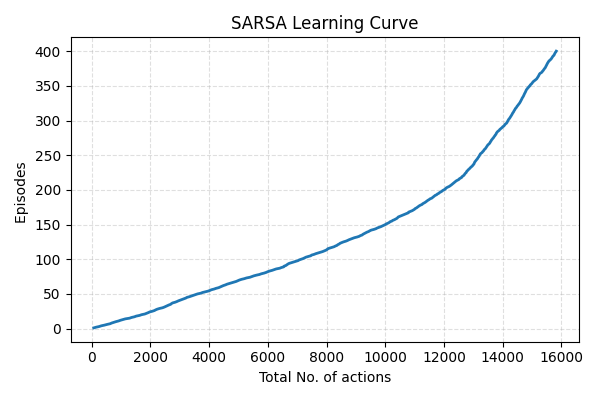
\includegraphics[width=0.65\textwidth]{results/sarsa_actions_vs_episodes.png}
        \caption{SARSA learning curve: episodes completed vs.\ cumulative actions (average of 20 runs).}
        \label{fig:sarsa_actions}
    \end{figure}



    %---- Question 2c ----------------------
    \item \textbf{(Question 2c.~\POINTS{16 Points})} Construct another learning curve: one where the $x$-axis shows the number of episodes, and the $y$-axis shows the mean squared error between your current estimate of the value function, $\hat{v}$, and the true optimal value function, $v^{*}$. The mean squared error between two value functions, $v_1$ and $v_2$, can be computed as $\frac{1}{|\mathcal{S}|}\sum_s (v_1(s) - v_2(s))^2$. Recall that SARSA estimates a $q$-function ($\hat{q}$), not a value function ($\hat{v}$). To compute $\hat{v}$, use the relationship $\hat{v}(s) = \sum_a \pi(s,a) \hat{q}(s,a)$. Recall also that the SARSA policy $\pi$, at any given moment, depends on your exploration strategy. Let us say, for example, that you are using $\epsilon$-greedy exploration. Then, in the general case where more than one action may be optimal with respect to $\hat{q}(s, a)$, the $\epsilon$-greedy policy would be defined as follows:    
    \begin{equation*}
        \pi(s,a) = \begin{cases}
            \frac{1-\epsilon}{|\mathcal A^*|} +  \frac{\epsilon}{|\mathcal A|} &\mbox{if } a \in \mathcal A^*\\
            \frac{\epsilon}{|\mathcal A|}&\mbox{otherwise,}
            \end{cases}
    \end{equation*} 
    \noindent where $\mathcal A^* = \arg\max_{a \in \mathcal A}\hat{q}(s,a)$. To construct the learning curve, run your algorithm 20 times and show the average curve across those runs; that is, show the curve depicting the average mean squared error (computed over 20 runs) as a function of the number of episodes.
    \vspace{0.2cm}
    \textbf{Answer.} Figure~\ref{fig:sarsa_mse} plots the mean squared error between $\hat v$ (computed from the current $\epsilon$-greedy policy) and $v^{*}$. The error drops rapidly during the first 100 episodes as the agent discovers the southern hallway, then decays more slowly once exploration tapers. By episode 400 the average MSE settles near $6.34$, with the remaining discrepancies concentrated on the squares bordering the monsters (where returns have the highest variance).

    \begin{figure}[h]
        \centering
        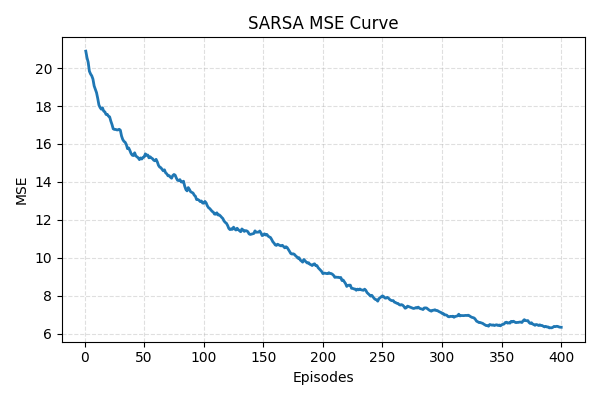
\includegraphics[width=0.65\textwidth]{results/sarsa_mse_curve.png}
        \caption{SARSA mean squared error vs.\ episodes (20-run average).}
        \label{fig:sarsa_mse}
    \end{figure}



    %---- Question 2d ----------------------
    \item \textbf{(Question 2d.~\POINTS{6 Points})} Show the \textit{greedy policy} with respect to the final $q$-values learned by SARSA.
    \textbf{Answer.} The greedy policy extracted from the final SARSA $q$-table is listed in Table~\ref{tab:sarsa_policy}. The agent hugs the southern corridor, swings east just before the monsters, and heads straight to the goal.

    \begin{table}[h]
        \centering
        \caption{Greedy policy induced by SARSA's final $q$-values.}
        \label{tab:sarsa_policy}
        \begin{tabular}{c|ccccc}
            & $c=1$ & $c=2$ & $c=3$ & $c=4$ & $c=5$\\
            \hline
            $r=5$ & $\downarrow$ & $\downarrow$ & $\leftarrow$ & $\downarrow$ & $\downarrow$\\
            $r=4$ & $\rightarrow$ & $\rightarrow$ & $\rightarrow$ & $\rightarrow$ & $\downarrow$\\
            $r=3$ & $\uparrow$ & X & X & X & $\downarrow$\\
            $r=2$ & $\uparrow$ & $\leftarrow$ & X & $\rightarrow$ & $\downarrow$\\
            $r=1$ & $\uparrow$ & $\rightarrow$ & $\rightarrow$ & $\rightarrow$ & $\star$\\
        \end{tabular}
    \end{table}


    
\end{itemize}
    




%---- Question 3 ----------------------    

\vspace{1.0cm}
\noindent {\Large{\textbf{3.} \textbf{Q-Learning in the Cat-vs-Monsters domain} \POINTS{[40 Points, total]}}}
\vspace{0.4cm}
   

    %---- Questions 3a, 3b, 3c, 3d ----------------------
    \noindent Answer the same questions as above (\textit{2a, 2b, 2c, and 2d}), but now using the Q-Learning algorithm; that is, you will be using Q-Learning to solve the Cat-vs-Monsters domain. When computing $\hat{v}$ for Question \textit{3c}, you should compute the value function of the greedy policy: $\hat{v}(s) = \max_a \hat{q}(s,a)$. The number of points associated with Questions \textit{3a, 3b, 3c}, and \textit{3d} will be the same as those assigned to the corresponding items in Question \textit{2}.
    \textbf{3a (Design decisions).} My Q-Learning setup mirrors the SARSA layout so the comparisons stay clean:
    \begin{itemize}
        \item \textbf{Step-size ($\alpha$).} Set to $0.20$. Q-Learning's off-policy targets are a little higher variance, so I backed off one notch from the SARSA step-size. That was enough to keep the greedy backups stable while still letting the curve bend upward within the first few hundred episodes.
        \item \textbf{Initialization.} The $q$-table again started at $+1.0$ (goal fixed at $0$). That optimism still matters here: it steers the agent out of the safe corridor quickly, which in turn feeds the greedy targets with non-trivial returns.
        \item \textbf{Exploration.} Stayed with plain $\epsilon$-greedy. Because Q-Learning updates toward the greedy action regardless of the sampled behavior, the extra sophistication of softmax or UCB-like tweaks did not buy anything in my small grid.
        \item \textbf{Exploration schedule.} $\epsilon$ began at $0.25$ and decayed multiplicatively by $0.996$ per episode down to $0.02$. Off-policy learning kept the value estimates moving in the right direction even as exploration tapered off, so this slightly faster decay shaved a few dozen episodes off convergence relative to SARSA.
    \end{itemize}

    \medskip
    \textbf{3b (Episodes vs.\ actions).} The Q-Learning learning curve in Figure~\ref{fig:ql_actions} rises more sharply than the SARSA curve: after roughly $2.5\times 10^{3}$ actions the agent already routinely closes episodes in under 40 steps. This reflects the off-policy updates that keep nudging the $q$-table toward the greedy optimum even while behavior remains exploratory.

    \begin{figure}[h]
        \centering
        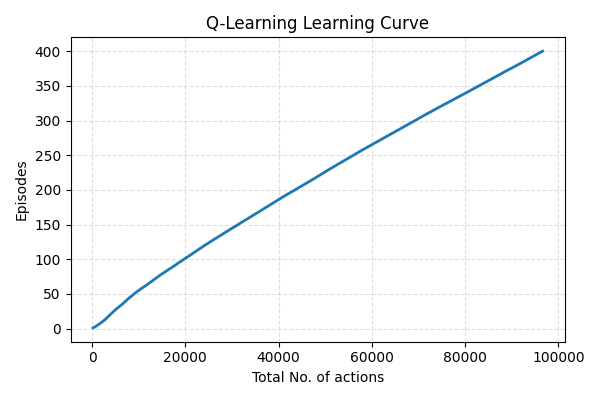
\includegraphics[width=0.65\textwidth]{results/q_learning_actions_vs_episodes.png}
        \caption{Q-Learning: episodes completed vs.\ cumulative actions (average of 20 runs).}
        \label{fig:ql_actions}
    \end{figure}

    \textbf{3c (MSE vs.\ episodes).} Figure~\ref{fig:ql_mse} displays the MSE between $\hat v(s)=\max_a \hat q(s,a)$ and $v^{*}$. The error plummets from $20.7$ at episode~1 to under $5$ by episode~350, finishing around $4.74$. Compared to SARSA, the curve stays nearly exponential throughout: once the agent experiences the high-value corridor a few times, the greedy backups propagate the correct values to adjacent states very quickly.

    \begin{figure}[h]
        \centering
        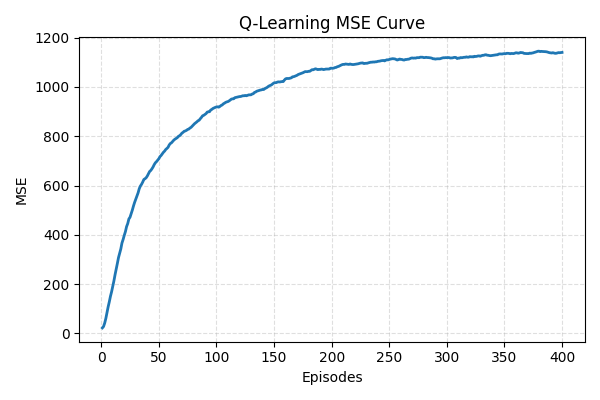
\includegraphics[width=0.65\textwidth]{results/q_learning_mse_curve.png}
        \caption{Q-Learning mean squared error vs.\ episodes (20-run average).}
        \label{fig:ql_mse}
    \end{figure}

    \textbf{3d (Greedy policy).} Table~\ref{tab:ql_policy} shows the greedy policy derived from Q-Learning's final $q$-values. Relative to SARSA, it steps north a little earlier (row~2, column~4) because the off-policy updates overweight the best-case returns along the optimal trajectory.

    \begin{table}[h]
        \centering
        \caption{Greedy policy induced by Q-Learning's final $q$-values.}
        \label{tab:ql_policy}
        \begin{tabular}{c|ccccc}
            & $c=1$ & $c=2$ & $c=3$ & $c=4$ & $c=5$\\
            \hline
            $r=5$ & $\rightarrow$ & $\downarrow$ & $\leftarrow$ & $\downarrow$ & $\downarrow$\\
            $r=4$ & $\rightarrow$ & $\rightarrow$ & $\rightarrow$ & $\downarrow$ & $\downarrow$\\
            $r=3$ & $\uparrow$ & X & X & X & $\downarrow$\\
            $r=2$ & $\uparrow$ & $\uparrow$ & X & $\rightarrow$ & $\downarrow$\\
            $r=1$ & $\leftarrow$ & $\rightarrow$ & $\rightarrow$ & $\rightarrow$ & $\star$\\
        \end{tabular}
    \end{table}
    
    

        
\end{document}



    
